\documentclass[border=10pt]{standalone}

\usepackage{tikz}
\usepackage{tikzsymbols}
\usetikzlibrary{calc,patterns,shapes.geometric}

\def\centerarc[#1](#2)(#3:#4:#5){\draw[#1] ($(#2)+({#5*cos(#3)},{#5*sin(#3)})$) arc (#3:#4:#5);}

\begin{document}
	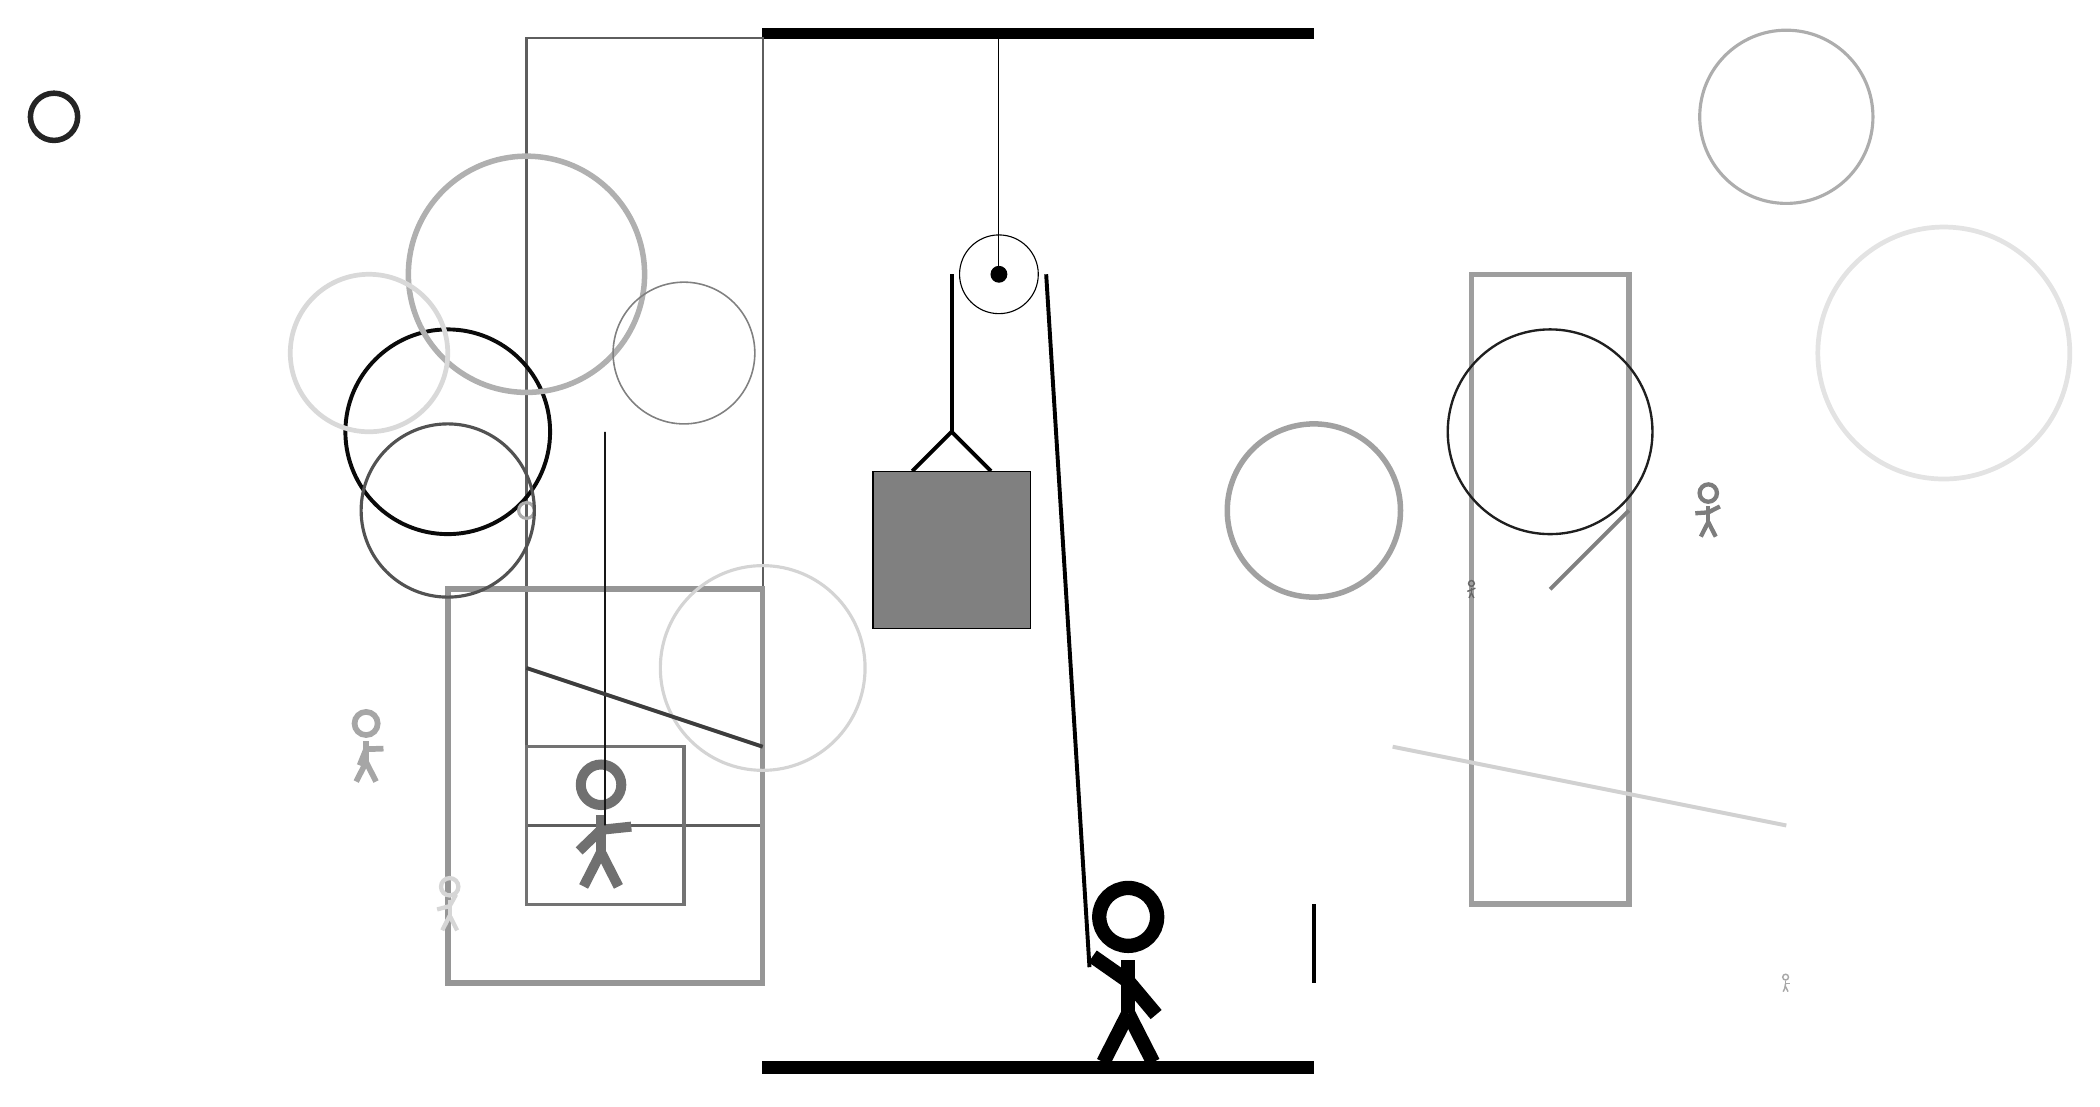
\begin{tikzpicture}
		%%%%% START %%%%%
		
		\draw[fill=black] (-2, 10) rectangle (5, 10.125);
		
		\draw (1, 7) circle (0.5);
		\draw[fill=black] (1, 7) circle (0.1);
		\draw (1, 10) -- (1, 7);
		
		\draw[line width=0.5mm] (-0.1, 4.5) -- (0.4, 5.0) -- (0.9, 4.5);
		\draw[fill=black!50] (-0.6, 4.5) rectangle (1.4, 2.5);
		
		\draw[line width=0.3mm, color=black!63] (-2, 10) rectangle (-5, 0);
		
		\node[line width=0.7mm, color=black!56] at (-4, 0) {\Strichmaxerl[7][44][6]};
		\draw[line width=0.4mm, color=black!55] (-3, -1) rectangle (-5, 1);
		\draw[line width=0.7mm, color=black!41] (-2, 3) rectangle (-6, -2);
		\draw[line width=0.7mm, color=black!38] (7, -1) rectangle (9, 7);
		
		\draw [line width=0.5mm, color=black!96](-6, 5) circle (1.3);
		
		\draw [line width=0.4mm, color=black!33](-5, 4) circle (0.1);
		
		\draw[line width=0.5mm, color=black!18](6, 1) -- (11, 0);
		\node[line width=0.2mm, color=black!16] at (-6, -1) {\Strichmaxerl[3][15][61]};
		\draw[line width=0.2mm, color=black!91] (-4, 5) rectangle (-4, 0);
		\draw [line width=0.7mm, color=black!31](-5, 7) circle (1.5);
		\draw [line width=0.6mm, color=black!11](13, 6) circle (1.6);
		\node[line width=0.7mm, color=black!60] at (7, 3) {\Strichmaxerl[1][20][24]};
		
		\draw[line width=0.5mm, color=black!100] (5, -1) rectangle (5, -2);
		\node[line width=0.3mm, color=black!51] at (10, 4) {\Strichmaxerl[3][4][27]};
		\draw [line width=0.4mm, color=black!17](-2, 2) circle (1.3);
		
		\draw [line width=0.7mm, color=black!86](-11, 9) circle (0.3);
		
		\draw [line width=0.6mm, color=black!15](-7, 6) circle (1.0);
		\draw[line width=0.5mm, color=black!76](-2, 1) -- (-5, 2);
		\draw [line width=0.4mm, color=black!32](11, 9) circle (1.1);
		\draw [line width=0.7mm, color=black!37](5, 4) circle (1.1);
		\draw[line width=0.5mm, color=black!50](9, 4) -- (8, 3);
		\draw [line width=0.2mm, color=black!50](-3, 6) circle (0.9);
		\node[line width=0.4mm, color=black!35] at (-7, 1) {\Strichmaxerl[4][68][2]};
		\draw [line width=0.4mm, color=black!68](-6, 4) circle (1.1);
		
		\draw [line width=0.3mm, color=black!88](8, 5) circle (1.3);
		
		\node[line width=0.5mm, color=black!34] at (11, -2) {\Strichmaxerl[1][79][0]};
		
		\draw[line width=0.5mm] (0.4, 7) -- (0.4, 5.0);
		\centerarc[line width=0.5mm](1, 7)(0:180:0.6);
		\draw[line width=0.5mm](1.6, 7) -- (2.15, -1.8);
		
		\node at (2.6, -1.9) {\Strichmaxerl[10][-35][-50]};
		
		\draw[fill=black] (-2, -3) rectangle (5, -3.15);
		
		%%%%% END %%%%%
	\end{tikzpicture}
\end{document}